%!TEX root = ../../dissertation.tex
\begin{savequote}[75mm]
Why are people still telling me what to do? I don't want to do anything. What is the thing I should copy-paste to my agent? 
\qauthor{Andrej Karpathy}
\end{savequote}

\chapter{Automating FEP calculations with AI Agents}
\label{ch:automating-abfes-with-ai-agents}
In the previous chapters, we examined errors in ABFEP calculations arising from insufficient sampling and improper simulation setup. Alongside these errors, another major barrier to the wider adoption of FEP is its labour-intensive setup process. LLM-based coding agents, which are increasingly capable of performing scientific workflows, promise to lower this barrier. However, despite their potential to accelerate FEP and molecular dynamics (MD) research more broadly, their reliability on realistic MD tasks remains poorly characterised, owing to the lack of rigorous benchmarks. In the absence of such benchmarks, researchers cannot reliably integrate coding agents into FEP and broader MD workflows.

To address this gap, we introduce MDArena, a benchmark of 50 containerised tasks drawn from active biomolecular simulation projects. The tasks span 29 molecular systems and seven task types, including trajectory analysis, complex system preparation, free-energy calculations, and enhanced sampling. We evaluate 18 coding agent configurations, released between July 2025 and November 2026 and show that the latest frontier models score consistently high on easy and medium tasks and show substantial gains on hard tasks. However, failures persist in tasks relating to membrane-protein system preparation and alchemical free-energy setup. MDArena thus exposes the gap between coding agents as supervised assistants and as autonomous MD researchers, and provides a reproducible, extensible platform for tracking progress in closing it.



\section{Introduction}

Molecular dynamics (MD) has become central to modern biomolecular research. Over the past decades, it has been widely used across scientific disciplines and has delivered insights into molecular mechanisms, dynamics, and functions.\cite{hollingsworth2018molecular,huggins2019biomolecular} While its underlying theory is well established, carrying out a scientifically defensible MD workflow remains technically demanding, as it requires meticulous system preparation, parameterization, selection of appropriate sampling protocols, and analysis tailored to the scientific question. These tasks require substantial expertise and are often repeated across systems and projects, creating a strong incentive to automate their execution.

Recent advances in large language models (LLMs) and coding agents offer a promising route toward such automation.\cite{zhao2023survey,liu2024large} MD is well suited to agentic assistance because its workflows are mature, modular, and supported by a variety of well-documented simulation and analysis software.\cite{abraham2015gromacs,eastman2023openmm,michaud2011mdanalysis} Equipped with language-based reasoning and the ability to interact directly with computational environments, an agent could in principle translate a scientific objective into an actionable workflow, orchestrate available tools, and iteratively adapt protocols given intermediate results or failures. Still, reliable automation of MD workflows, and its evaluation, are non-trivial. The challenge lies in the sequential coupling between workflow stages: an error introduced at one step, such as an incorrect protonation state or ligand topology, can propagate and invalidate subsequent calculations, wasting expensive compute. Compounding this problem, many mistakes are silent, as a successfully executed simulation may still produce plausible results even when the underlying system or protocol is flawed. A benchmark must therefore assess not only whether an agent can execute MD software successfully, but also whether its workflow and outputs are scientifically valid, especially in realistic scenarios that mirror actual research projects or drug-discovery campaigns. Existing benchmarks and evaluations often fall short on this front,\cite{kumar2026mdgym,campbell2026mdcrow,guilbert2025dynamate,chandrasekhar2025namdagent,zhao2026polyjarvis,vriza2026multiagentic} relying on isolated toy problems and narrow research contexts while providing limited support for evaluating the validity of an agent's workflow.

We therefore introduce MDArena, an executable benchmark of 50 expert-curated, containerized tasks drawn directly from active research projects. Spanning three difficulty levels, the tasks cover 29 diverse biomolecular systems and 18 simulation software packages, and include membrane-protein preparation, parameterization of non-standard residues, free energy methods, enhanced-sampling protocols, quantum-chemistry workflows, and bespoke analysis across diverse research contexts. 

We track the performance of agents released between July 2025 and November 2026 and show that frontier agents can autonomously perform MD tasks, ranging from simple analysis to complex membrane-protein FEP system preparation. The best models succeed across a broad range of tasks, although some failures persist across repeated attempts. Claude Opus-5.5 achieved the highest strict pass rate at 94.7\% (142 of 150 trials), while GPT-6.1 Sol was the most cost-effective configuration, with an 88.0\% strict pass rate (132 of 150 trials) and a cost of \$0.53 per strict pass, compared with \$0.91 for Opus-5.5. Both are closely followed by Gemini-4 Argon and open-source models such as GLM. Together, these results characterize the state of the art in agentic assistance for MD. The strongest agents evaluated are ready for adoption in production workflows, provided that edge cases are documented and requirements are stated explicitly.

\subsection{Related Works}

The growing ubiquity of AI agents in scientific computing has driven a parallel effort to benchmark them on realistic scientific workflows, and MD is no exception. Yet most existing benchmarks remain narrow in scope and fail to capture the breadth of high-level tasks relevant to MD workflows. Broader scientific benchmarks such as SciCode and ScienceAgentBench evaluate research-oriented programming and data analysis, while Corral combines executable scientific tasks, including molecular simulation, with analysis of agents' scientific reasoning. MDCrow\cite{campbell2026mdcrow} was the first to evaluate LLM agents with 40+ tools on 25 MD tasks, but its scope is limited and modern coding agents now nearly saturate the suite. NAMD-Agent\cite{chandrasekhar2025namdagent} followed, automating the CHARMM-GUI interface\cite{jo2008charmm} via Gemini\cite{team2023gemini} and Selenium, but it serves primarily as a system demonstration and introduces no accompanying benchmark. ChemGraph\cite{pham2026chemgraph} applies multi-agent orchestration to computational chemistry workflows, including geometry optimization, reaction enthalpy, and Gibbs free energy. It reports 100\% accuracy on all tasks tested, although the task suite is small and focuses on textbook-scale problems. DynaMate\cite{guilbert2025dynamate} was the first to target biomolecular MD with realistic tasks, evaluating a 12-system benchmark and automating the industry-relevant MM/GBSA binding-affinity estimation, though it remains a system demonstration rather than a generalizable agent benchmark. MDForge\cite{wang2026mdforge} introduces an LLM agent that uses multi-agent debate to design free energy pipelines. Ma et al.'s MDAgent and PRAXIS-MD integrate research planning, simulation, and interpretation through reusable skills and memory, including membrane-protein applications. Despite covering a wide range of workflows, PRAXIS-MD includes only 9 cases and is used predominantly to benchmark its own workflow rather than frontier coding agents. MDAgent2\cite{shi2026mdagent2} contributes MD-EvalBench, the first dedicated MD benchmark suite, alongside a domain-adapted Qwen3-8B model\cite{yang2025qwen3} trained via continued pretraining, supervised fine-tuning, and reinforcement learning with execution as the reward signal. Its scope, however, is restricted to LAMMPS\cite{thompson2022lammps} code generation, with no biomolecular tasks. Similarly, LAMMPS-Agents\cite{vriza2026multiagentic} enables end-to-end LAMMPS workflows for inorganic materials, and PolyJarvis\cite{zhao2026polyjarvis} extends this direction to polymer MD by orchestrating polymer MD toolkits via Model Context Protocol (MCP) servers. MDGym\cite{kumar2026mdgym} is a dedicated benchmark in this line, evaluating agents on GROMACS\cite{abraham2015gromacs} and LAMMPS\cite{thompson2022lammps} workflows rather than merely demonstrating agent capability. It provides an important foundation, while leaving several opportunities for broader evaluation. Its biomolecular tasks score agents against simulation output directly, which can conflate protocol correctness with sampling noise. The suite focuses on simulation execution given pre-built structures and topologies, leaving system preparation and parameterization for future extension, and it concentrates on well-known soluble protein systems. Additionally, tasks are framed as property-prediction problems with fixed accuracy thresholds (e.g., 5\% deviation), an approach that could be complemented by grading strategies better suited to settings without a well-defined ground truth. Finally, the reported failure-mode taxonomy is a useful starting point that could be complemented by more fine-grained, case-level analysis.



MDArena departs from these works along four axes:
\begin{enumerate}
    \item Provenance: Tasks are drawn from active research projects in a working MD group rather than authored as benchmark artifacts.
    \item Extensibility: Tasks are implemented in the harbor evaluation framework, allowing continual addition of novel research workflows as they arise. 
    \item Scope: coverage extends beyond prior work into alchemical free-energy perturbation (FEP)\cite{mey2020best} workflows, membrane-protein systems, protein-ligand complexes, and enhanced-sampling methods such as replica exchange of expanded ensembles (REXEE)\cite{hsu2024replica} and alchemical metadynamics \cite{hsu2023alchemical}.
    \item Evaluation: agent outputs and execution trajectories are graded with a dual-pronged scheme that combines human-authored, criterion-anchored rubrics with deterministic correctness checks designed to catch subtle but common agent errors that rubric grading alone can miss
\end{enumerate}
Together, these yield a more robust and diagnostically informative evaluation than execution- or output-matching alone.

\begin{table}[!htbp]
  \centering
  \caption[Positioning of MDArena relative to representative systems.]{Positioning of MDArena relative to representative agentic molecular-simulation and computational-chemistry systems. $\checkmark$, $\circ$, and $\times$ denote yes, partial or limited coverage, and no, respectively.}
  \label{tab:mdarena-positioning}
  \small
  \renewcommand{\arraystretch}{1.15}
  \begin{tabular*}{\textwidth}{@{\extracolsep{\fill}}lcccc@{}}
    \hline
    System or benchmark & \shortstack{Biomol.\\MD} & \shortstack{Exec.\\workflows} & Multipackage & \shortstack{Research\\provenance} \\
    \hline
    MDCrow~\cite{campbell2026mdcrow} & $\checkmark$ & $\checkmark$ & $\circ$ & $\circ$ \\
    NAMD-Agent~\cite{chandrasekhar2025namdagent} & $\checkmark$ & $\checkmark$ & $\times$ & $\circ$ \\
    DynaMate~\cite{guilbert2025dynamate} & $\checkmark$ & $\checkmark$ & $\circ$ & $\circ$ \\
    PolyJarvis~\cite{zhao2026polyjarvis} & $\times$ & $\checkmark$ & $\times$ & $\circ$ \\
    LAMMPS-Agents~\cite{vriza2026multiagentic} & $\times$ & $\checkmark$ & $\times$ & $\circ$ \\
    ChemGraph~\cite{pham2026chemgraph} & $\circ$ & $\circ$ & $\checkmark$ & $\circ$ \\
    MD-EvalBench~\cite{shi2026mdagent2} & $\times$ & $\circ$ & $\times$ & $\circ$ \\
    MDGym~\cite{kumar2026mdgym} & $\circ$ & $\checkmark$ & $\circ$ & $\circ$ \\
    MDArena & $\checkmark$ & $\checkmark$ & $\checkmark$ & $\checkmark$ \\
    \hline
  \end{tabular*}
\end{table}

\section{Methods}

\subsection{Task selection and curation}

MDArena was constructed from more than 100 candidate tasks contributed by domain experts from the Biggin Group to reflect the diversity and difficulty of problems encountered in research projects and drug discovery efforts. We screened the candidates for scientific relevance, technical substance, and complementarity, yielding an initial release of 50 tasks. The collection deliberately includes long-horizon workflows, underspecified problems requiring scientific judgements, and negative examples where the requested action is impossible or scientifically inappropriate. Its aggregate composition is shown in Figure~\ref{fgr:task-types}. Each task was assigned an easy, medium, or hard difficulty label by the task author and subsequently reviewed based on the workflow length, required domain knowledge, and technical complexity. The current benchmark comprises 10 easy, 24 medium and 16 hard tasks.


\begin{figure}[htbp]
\centering
  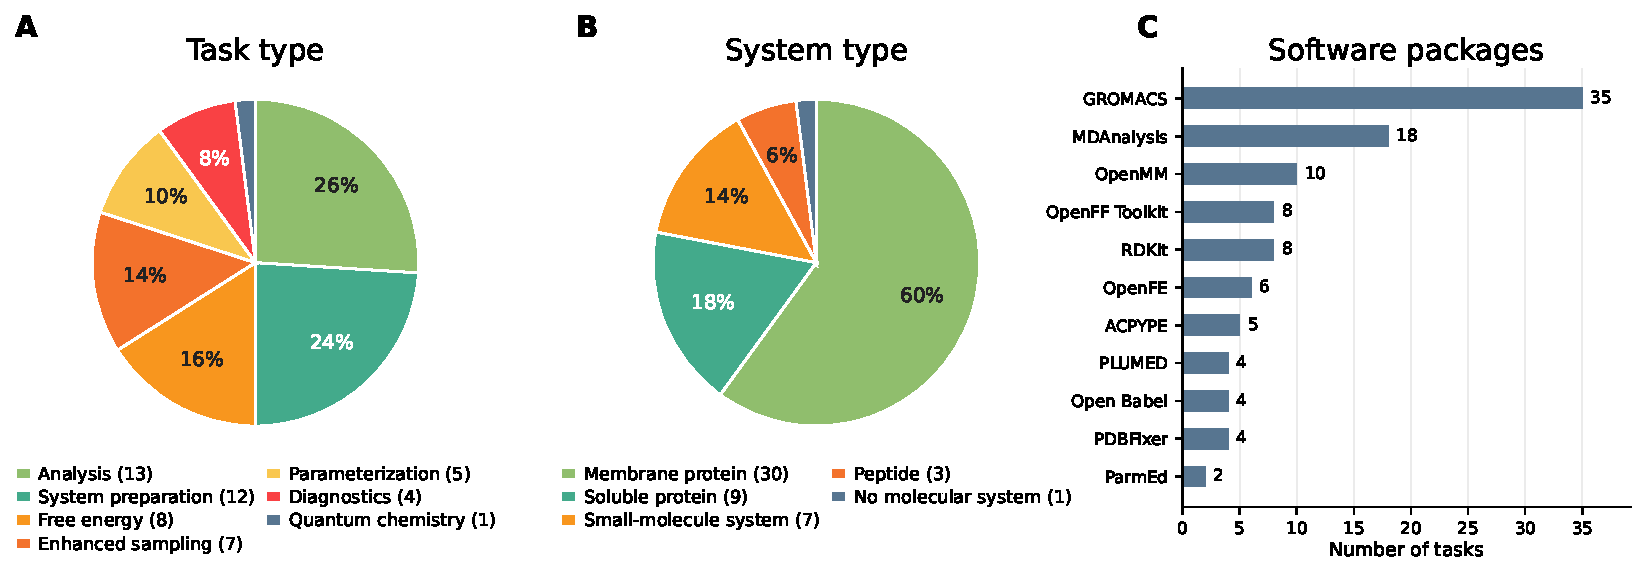
\includegraphics[width=\textwidth]{chapters/Ch7-Automating-ABFEP-calculations-with-AI-agents/figures/figure_1.pdf}
  \caption[MDArena dataset composition.]{Composition of the 50 MDArena tasks by (A) task type, (B) molecular system type, and (C) software package. Each task contributes once to panels A and B. The ``No molecular system'' category denotes a task operating only on a \mbox{GROMACS} MDP file. Tasks may use multiple packages, giving 111 task--package assignments across 18 packages in (C). Panel (C) shows the 11 packages used in at least two tasks; seven packages used in one task each are omitted for legibility.}
  \label{fgr:task-types}
\end{figure}


\subsection{Implementation}

 MDArena is implemented using the Harbor\cite{Harbor_Framework} evaluation framework, allowing researchers to readily evaluate their own agents and extend MDArena with new self-contained tasks. Each task runs in a dedicated Docker container \cite{moreau2023containers} and includes an executable reference solution that passes all correctness and process checks, confirming task solvability and validating that the verifier functions as intended. Command-line interfaces are provided for analyzing evaluation runs and collecting portable run records. To facilitate reproducibility and robustness, MDArena implements several safeguards. Task-content digests and run-metadata validation support checks of dataset integrity and evaluation configuration. Canary strings are embedded in task instructions, configuration files, verifiers, and reference-solution scripts to identify benchmark material and support the exclusion of our benchmark from future model-training corpora. Lastly, we implement continuous integration to run unit and regression tests for evaluation tools and task-specific verifiers, validate task structure, and check verifier dependencies in a containerized environment.

\begin{figure}[htbp]
\centering
  % Rearrange the four panels of the imported Figure 2 into a two-by-two grid.
  \begin{minipage}[t]{0.48\textwidth}
    \raggedright
    \textsf{\textbf{A}}\par
    \vspace{6pt}
    \centering
    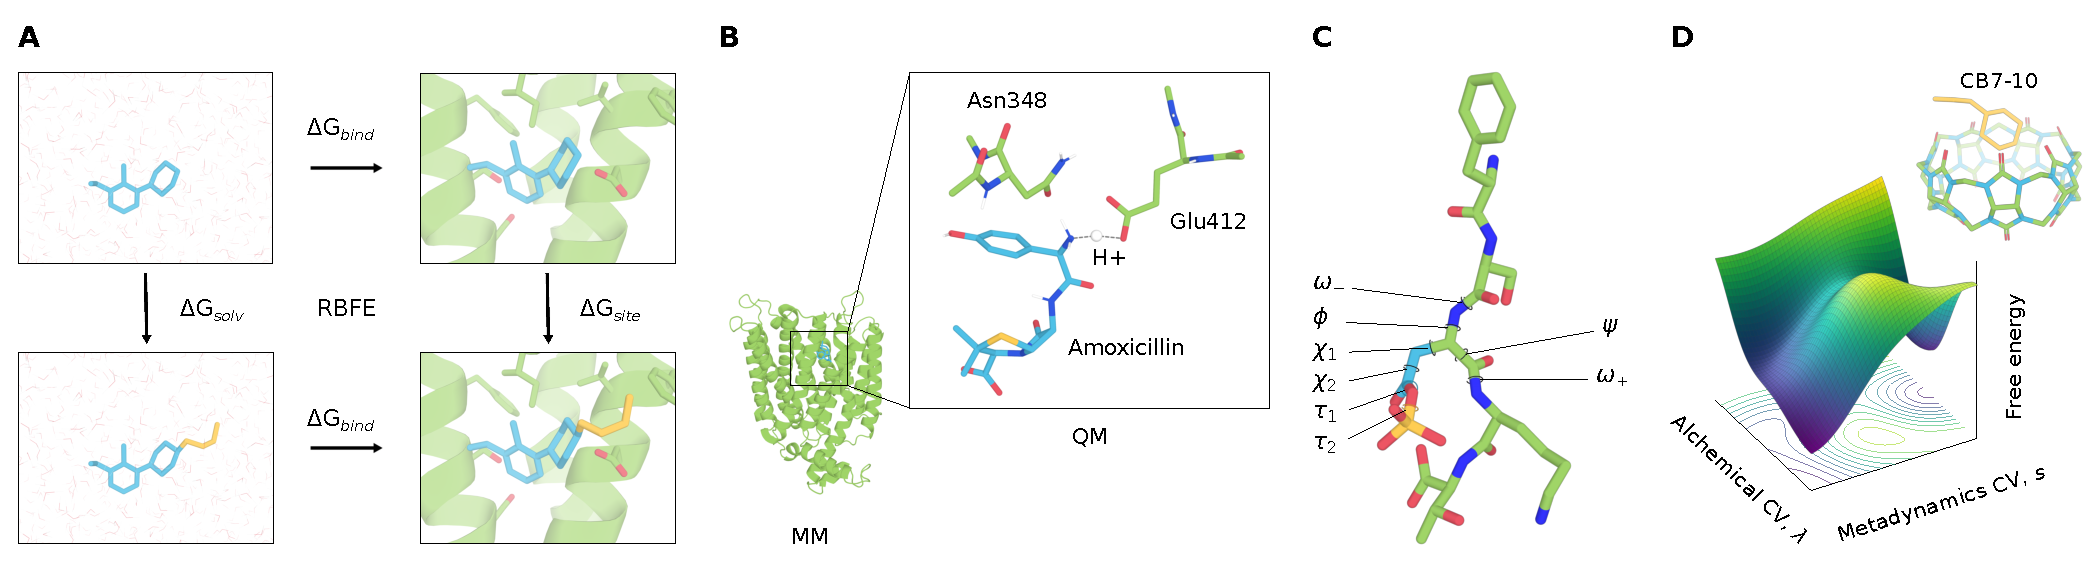
\includegraphics[width=\linewidth,height=0.72\linewidth,keepaspectratio,trim=8bp 8bp 683bp 34bp,clip]{chapters/Ch7-Automating-ABFEP-calculations-with-AI-agents/figures/representative_tasks_source.pdf}
  \end{minipage}\hfill
  \begin{minipage}[t]{0.48\textwidth}
    \raggedright
    \textsf{\textbf{B}}\par
    \vspace{6pt}
    \centering
    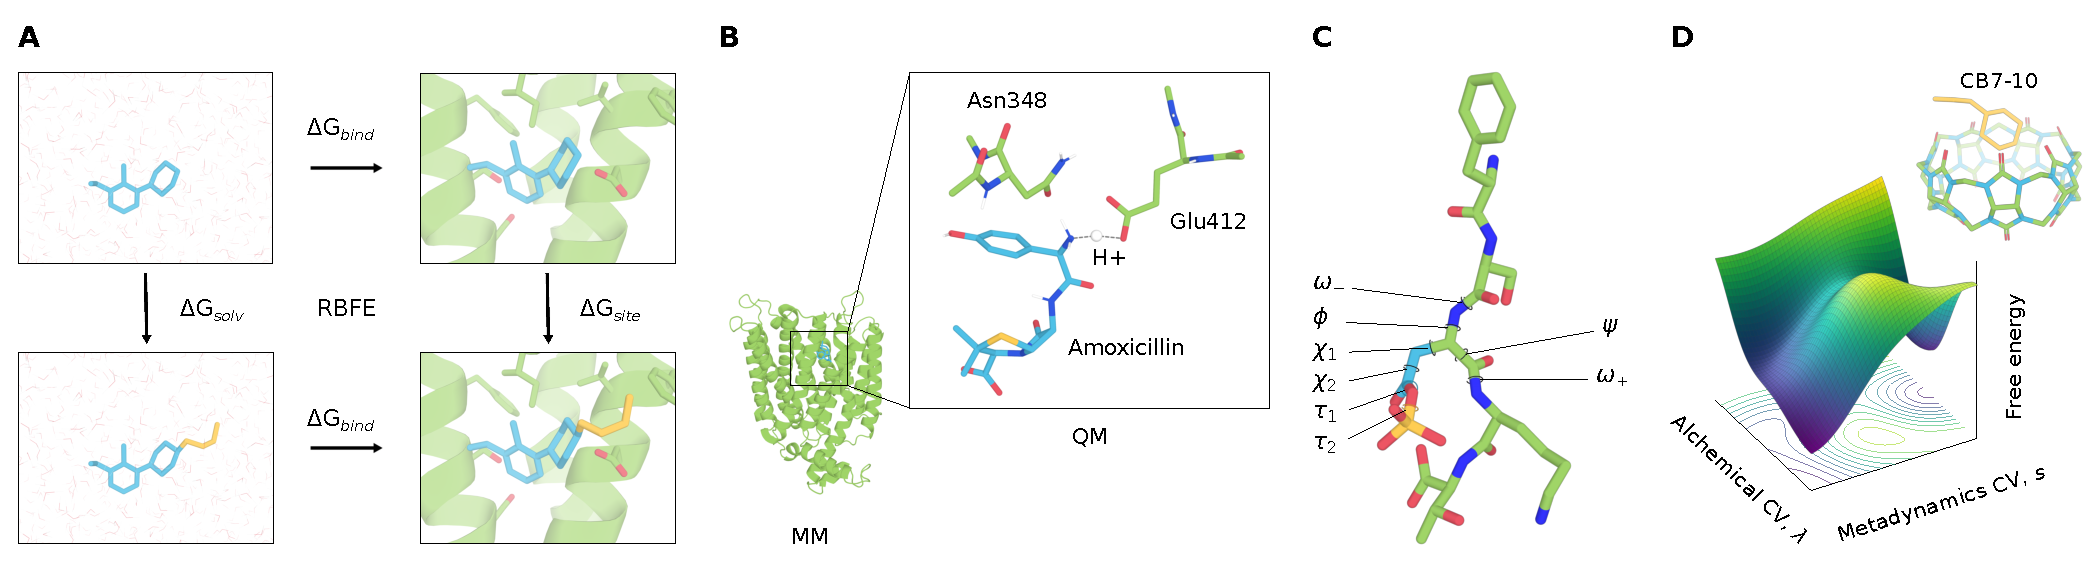
\includegraphics[width=\linewidth,height=0.72\linewidth,keepaspectratio,trim=344bp 8bp 398bp 34bp,clip]{chapters/Ch7-Automating-ABFEP-calculations-with-AI-agents/figures/representative_tasks_source.pdf}
  \end{minipage}\par
  \vspace{12pt}
  \begin{minipage}[t]{0.48\textwidth}
    \raggedright
    \textsf{\textbf{C}}\par
    \vspace{6pt}
    \centering
    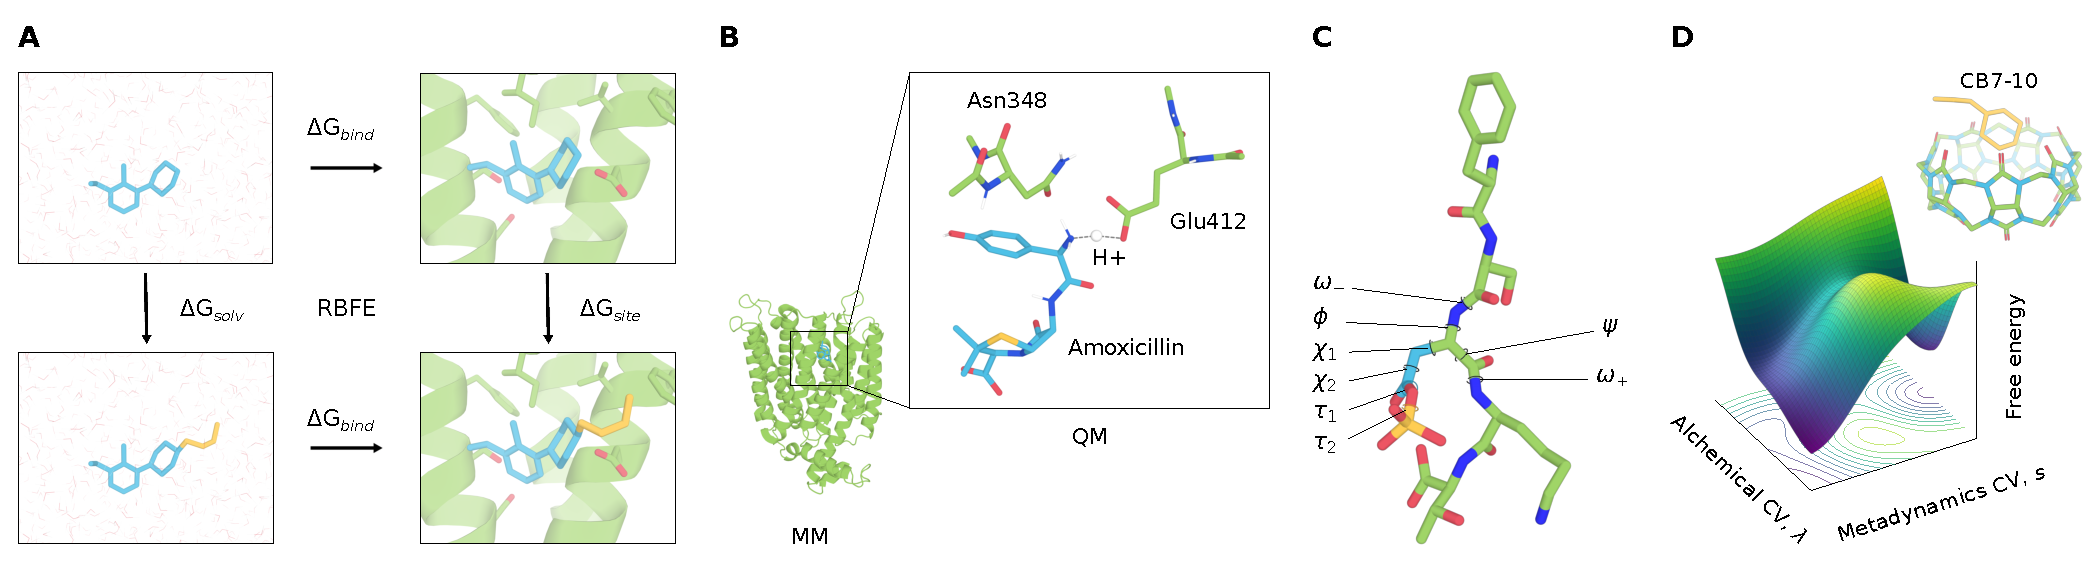
\includegraphics[width=\linewidth,height=0.72\linewidth,keepaspectratio,trim=629bp 8bp 226bp 34bp,clip]{chapters/Ch7-Automating-ABFEP-calculations-with-AI-agents/figures/representative_tasks_source.pdf}
  \end{minipage}\hfill
  \begin{minipage}[t]{0.48\textwidth}
    \raggedright
    \textsf{\textbf{D}}\par
    \vspace{6pt}
    \centering
    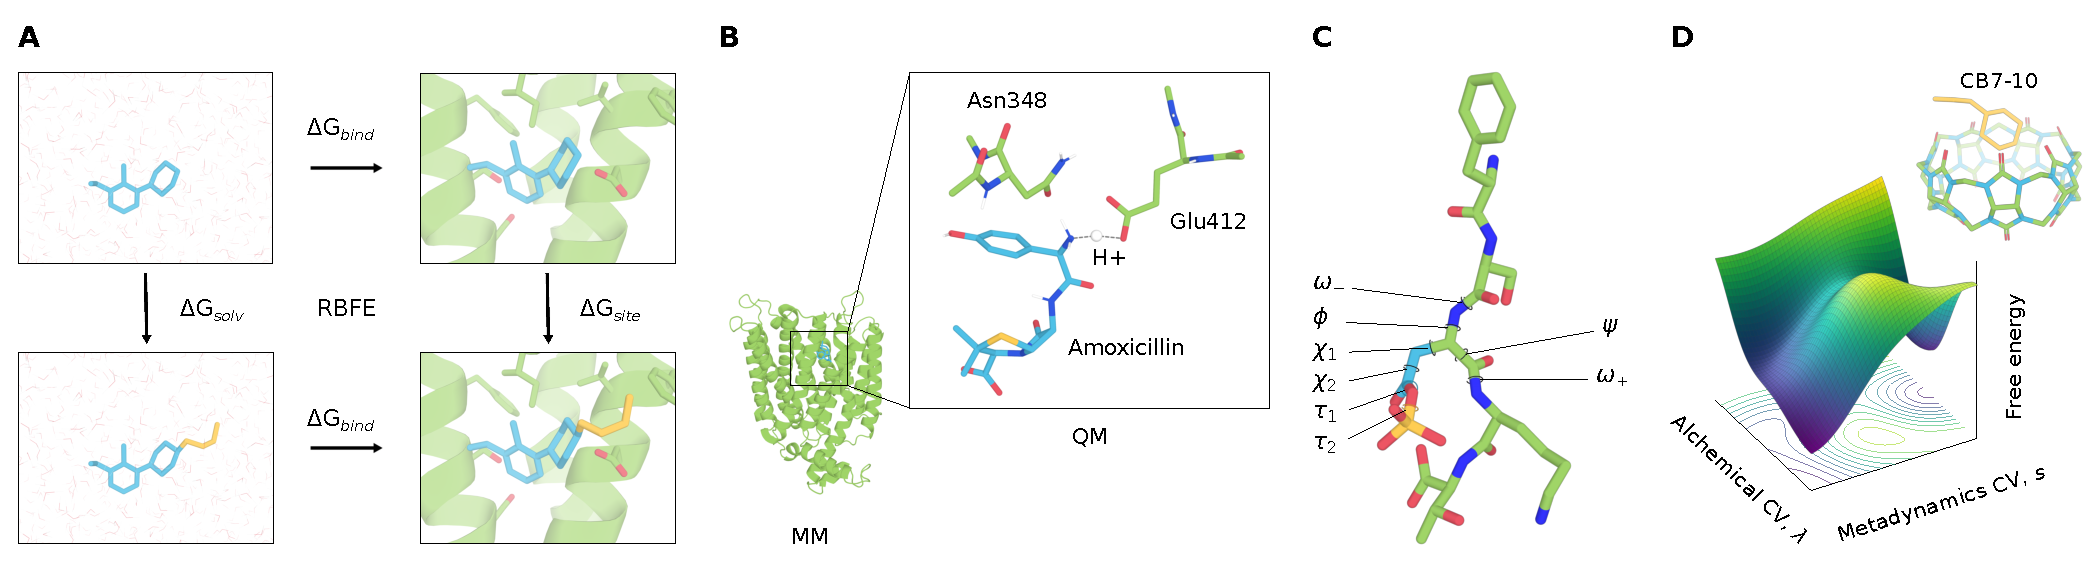
\includegraphics[width=\linewidth,height=0.72\linewidth,keepaspectratio,trim=801bp 8bp 8bp 34bp,clip]{chapters/Ch7-Automating-ABFEP-calculations-with-AI-agents/figures/representative_tasks_source.pdf}
  \end{minipage}
  \caption[Representative tasks and systems in MDArena.]{Representative tasks and systems in MDArena. (A) Planning a relative binding free-energy network for GPCR ligands using OpenFE (Task~33). (B) Constructing a PepT2--amoxicillin QM cluster for a proton-transfer scan in ORCA (Task~38). (C) Extending CHARMM36 to parameterize a pAsp-containing peptide (Task~47). (D) Performing alchemical metadynamics to estimate the absolute binding free energy of a host--guest complex (Task~48).}
\end{figure}
 
\subsection{Verification}

As molecular simulations are inherently stochastic and often lack a unique ground truth, \cite{wan2021uncertainty,communicationsbiology2023checklist} MDArena focuses primarily on stages such as system preparation, simulation configuration, and post-simulation analysis, where in fact much of the technical difficulty of an MD workflow lies and where outputs can often be evaluated deterministically. Each executed task is evaluated by a two-part verifier with Deterministic and Process checks. 

\textbf{Correctness checks} are deterministic examinations of whether the resulting artifacts satisfy task-specific numerical, structural, and software-level requirements. They include scored checks that assess artifact content and sanity checks that carry no correctness weight, such as file-existence checks. Where appropriate, verification independently reconstructs preparation steps or inspects compiled simulation inputs and accommodates scientifically valid alternatives without requiring exact reproduction of the reference solution. All correctness checks have been validated through Oracle sweeps, which execute the reference solutions and check for full correctness scores, as well as Nop sweeps, which check that performing no operation receives zero correctness credit. These sweeps are complemented by targeted regression tests using valid and invalid artifacts. 

\textbf{Process checks}, on the other hand, complement deterministic checks and use an LLM judge to assess the agent’s execution trajectory against predefined criteria covering the scientific decisions and interpretations necessary for a valid solution. The corresponding correctness and process scores are computed as the weighted fractions of criteria satisfied. Together, these two scores distinguish valid solutions from superficially convincing workflows and reveal cases in which a sound process nevertheless produces an incorrect result

\begin{figure}[htbp]
\centering
  % Isolate the timeline from the original vector figure, removing its panel label.
  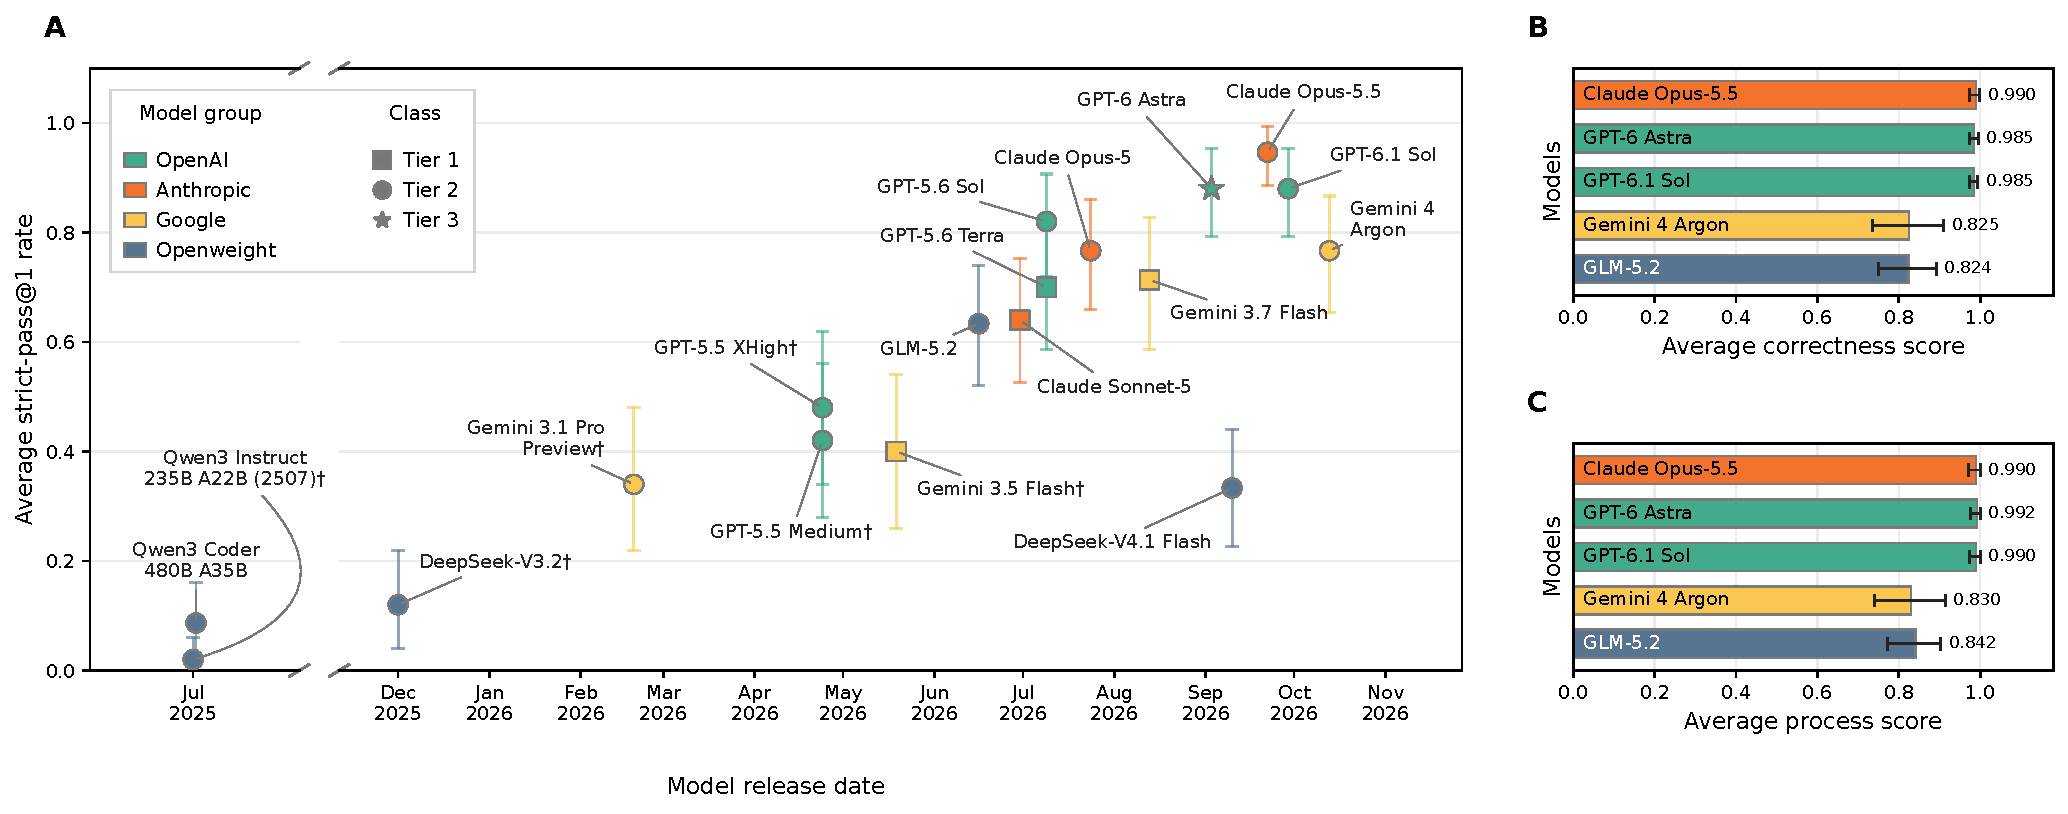
\includegraphics[width=\textwidth,trim=0bp 0bp 279bp 26bp,clip]{chapters/Ch7-Automating-ABFEP-calculations-with-AI-agents/figures/figure_2.pdf}
  \caption[Coding-agent strict-pass rates on MDArena.]{Mean Strict-Pass@1 against model release date on MDArena. A strict pass requires all correctness and process checks to pass. Error bars show 95\% task-bootstrap confidence intervals. Daggers mark v0.1.0 runs with one attempt per task; other runs use the v1 of the benchmark with three attempts per task.}
  \label{fig:model_performance}
  \label{fig:success-reward-triptych}
\end{figure}

\begin{figure}[htbp]
\centering
  % Crop the original score panels to matching sizes and place them side by side.
  \begin{minipage}[t]{0.48\textwidth}
    \raggedright
    \textsf{\textbf{A}}\par
    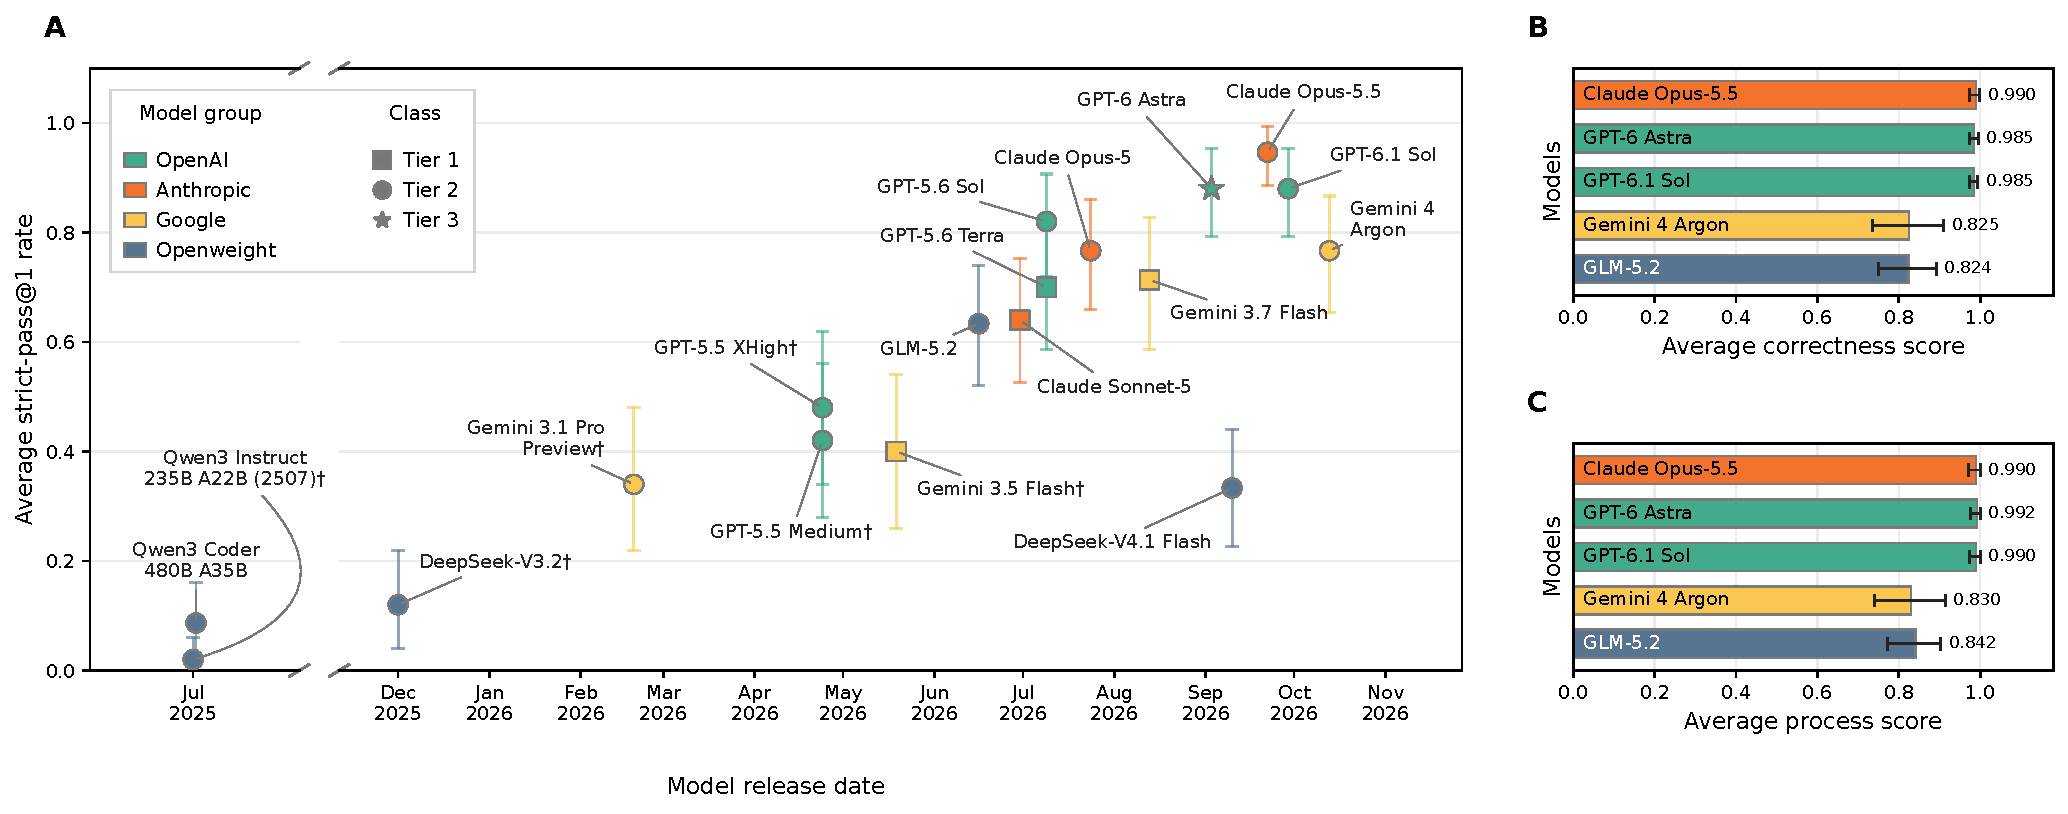
\includegraphics[width=\linewidth,trim=731bp 212bp 0bp 26bp,clip]{chapters/Ch7-Automating-ABFEP-calculations-with-AI-agents/figures/figure_2.pdf}
  \end{minipage}\hfill
  \begin{minipage}[t]{0.48\textwidth}
    \raggedright
    \textsf{\textbf{B}}\par
    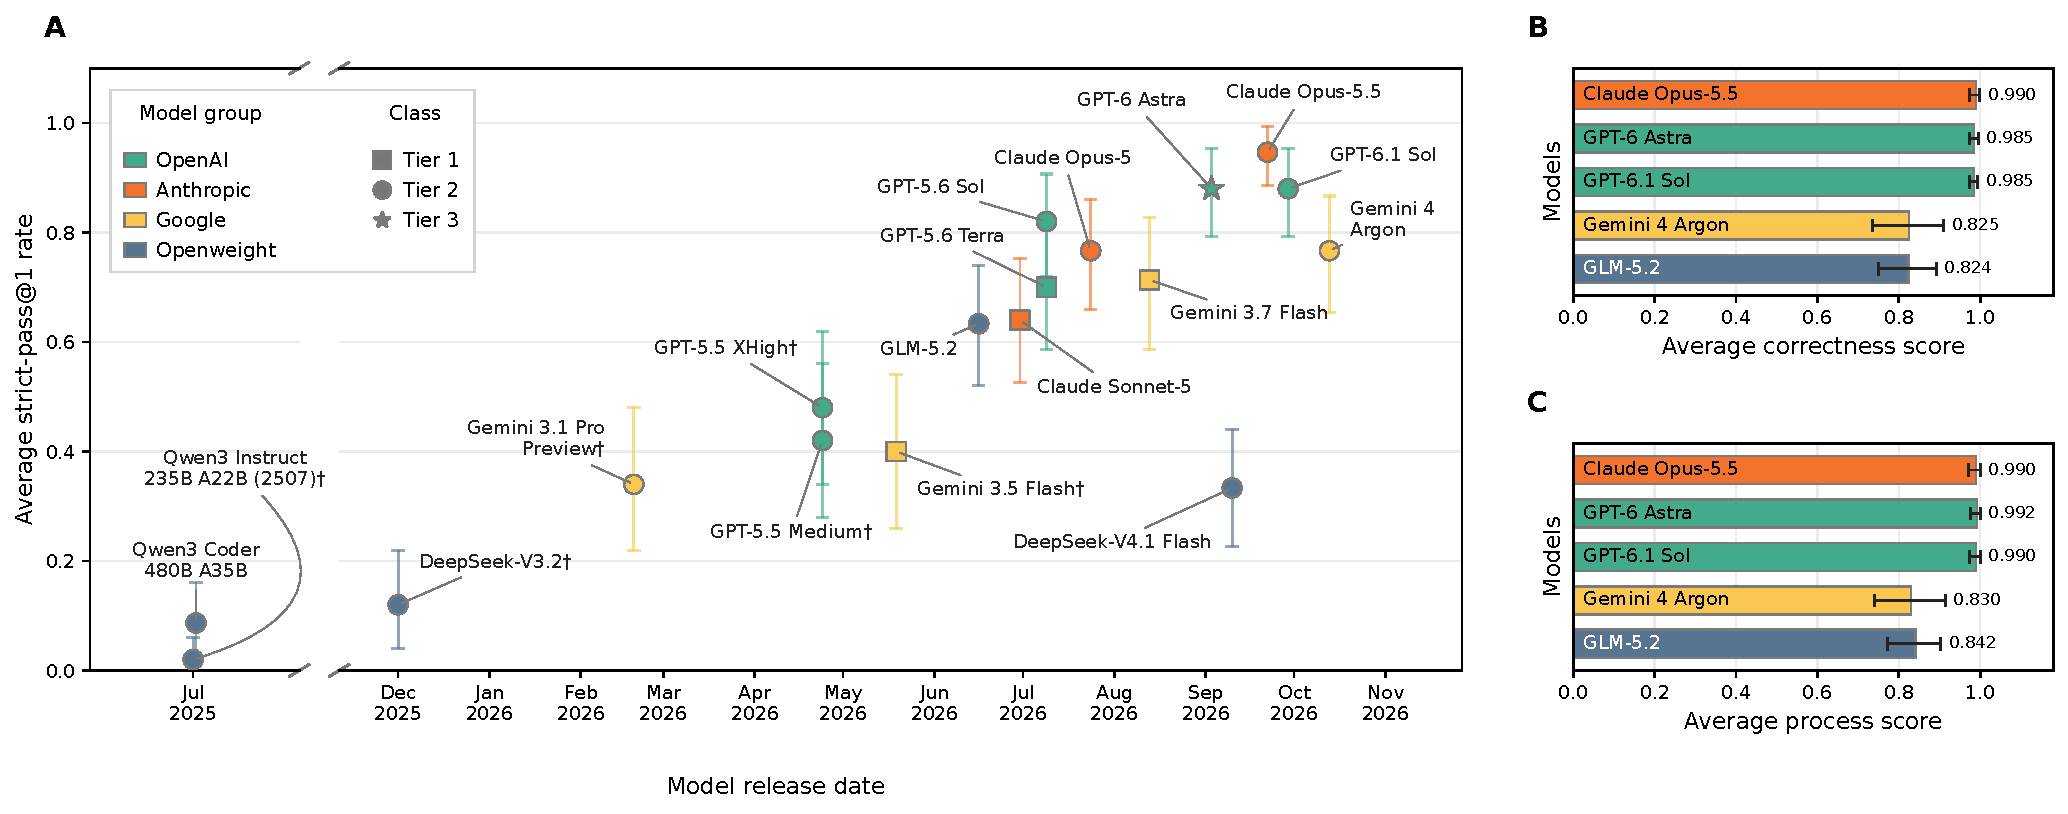
\includegraphics[width=\linewidth,trim=731bp 32bp 0bp 206bp,clip]{chapters/Ch7-Automating-ABFEP-calculations-with-AI-agents/figures/figure_2.pdf}
  \end{minipage}
  \caption[Coding-agent correctness and process scores on MDArena.]{Mean (A) correctness and (B) process scores on MDArena for five selected models. Error bars show 95\% task-bootstrap confidence intervals.}
  \label{fig:model_scores}
\end{figure}

\subsection{Experimental setup}


 We tracked the performance of frontier models from May 2026 onwards, covering both open-source and proprietary models from OpenAI (GPT-5.5 Medium and XHigh, GPT-5.6 Sol and Terra, GPT-6.1 Sol, and GPT Astra), Anthropic (Claude Opus-5 and Sonnet-5), Google (Gemini Flash 3.5, Pro 3.1, 3.7 Flash, and 4 Argon), DeepSeek (V3.2), Alibaba (Qwen3-235B and Qwen3 Coder 480B A35B), and Z.ai (GLM-5.2). In the main v1 evaluation, each configuration was evaluated in three independent trials on all 50 tasks. Claude Opus-5 was used as the process judge across all trials to ensure consistent grading. Tasks were executed in Docker containers with internet access, but GitHub and repository mirrors were blocked to prevent task lookup. Each task had access to 2–4 CPUs, 8 GB RAM, 10 GB storage, no GPUs, and a task-specific wall-clock limit ranging from 10 minutes to 2.5 hours given its computational requirements.

Check the difference between this and the original thing

\subsection{Evaluation metrics and statistical analysis}

For each configuration, the reported strict-pass@1 rate was calculated as the fraction of individual trials that pass all scored correctness and process checks:
\begin{equation}
  \text{Strict-Pass@1} = \frac{1}{NR} \sum_{i=1}^{N} \sum_{r=1}^{R} s_{ir},
\end{equation}
where $N$ is the number of tasks, $R$ is the number of replicates per task, and $s_{ir}$ equals one if replicate $r$ on task $i$ achieves a strict pass and zero otherwise. Mean correctness and process scores were calculated by averaging the corresponding scores across all trials. For configurations evaluated with three replicates per task, Pass@3 denotes the fraction of tasks with at least one strict pass, while Pass$^3$, as a repeatability measure, denotes the fraction with strict passes in all three replicates.

Timeouts and other runtime failures were retained as failed deliveries and assigned zero correctness and process scores in the adjusted metrics. Confidence intervals were computed as 95\% percentile bootstrap intervals from 2,000 resamples, sampling tasks rather than trials so that repeated attempts at one task were not treated as independent.

\section{Results and Discussion}

\subsection[Reliable execution of complex MD workflows]{Frontier coding agents can reliably execute complex molecular dynamics workflows}

Frontier LLMs have made a leap in capabilities over the past few months, and this is reflected in their MDArena scores (Figure~\ref{fig:model_performance}). In the initial v0.1.0 evaluation, Gemini 3.1 Pro Preview and GPT-5.5 (extra-high effort) achieved strict pass rates of 34\% and 48\%. The latest frontier models, however, perform substantially better: Gemini 4 Argon achieved 76.7\%, GPT-6.1 Sol achieved 88\%, while Claude Opus 5.5 was the overall best model, reaching 94.7\% and passing 49 of 50 tasks at least once across three attempts. These observations are consistent with documented improvements in reasoning efficiency and in persistent reasoning across extended interactions, which together enable more reliable execution of complex, long-horizon tasks such as those in MDArena. These results indicate that coding agents have now matured enough to be integrated into bounded MD research workflows. However, their performance on harder tasks remains fragile, requiring explicit scientific instructions and independent validation of outputs.


\subsection[Partial credit and strict task success]{High Partial-Credit Rewards Do Not Guarantee Strict Task Success}

Most frontier agents achieved consistently high partial-credit rewards, even on failed tasks, suggesting that most failures arise from minor errors rather than fundamental flaws in the workflow (Figure~\ref{fig:model_scores}). The latest closed frontier agents attained mean correctness and process rewards above 0.98, with Claude Opus 5.5 achieving the highest correctness (0.990) and GPT-6 Astra the highest process reward (0.992). These rewards substantially exceeded the corresponding Strict-Pass@1 rates, indicating that high partial credit does not necessarily translate into complete task success. Gemini 4 Argon and GLM 5.2 were notable exceptions, with lower mean rewards. This was largely attributable to trials that exceeded the time limit and terminated before completion, which were assigned a score of zero on both correctness and process checks. When the analysis was restricted to trials with a successful exit status, Gemini 4 Argon improved from 82.47\% to 97.69\% in correctness and from 82.99\% to 98.03\% in process, while GLM 5.2 improved from 82.37\% to 87.90\% in correctness and from 84.15\% to 90.04\% in process. The low correctness and process scores are therefore likely an artefact of the implementation and the OpenCode agent harness rather than of the models themselves.

Most models were run with three repeats to test repeatability. Claude Opus 5.5 passed 49/50 tasks at least once across three attempts (Pass@3) and 46/50 in all three attempts (Pass$^3$), while GPT-6.1 Sol and GPT-6 Astra each achieved identical Pass@3 and Pass$^3$ scores of 46/50 and 43/50, respectively. Gemini 4 Argon passed 42 tasks at least once and 34 on all three attempts, while GLM-5.2 passed 39 at least once and 24 on all three. Even the strongest configuration, Claude Opus 5.5, failed at least one attempt on four of the 50 tasks, underscoring the fragility of these models on harder tasks.

\begin{figure}[htbp]
\centering
  % Retain panels A and B together, with the full shared model legend below.
  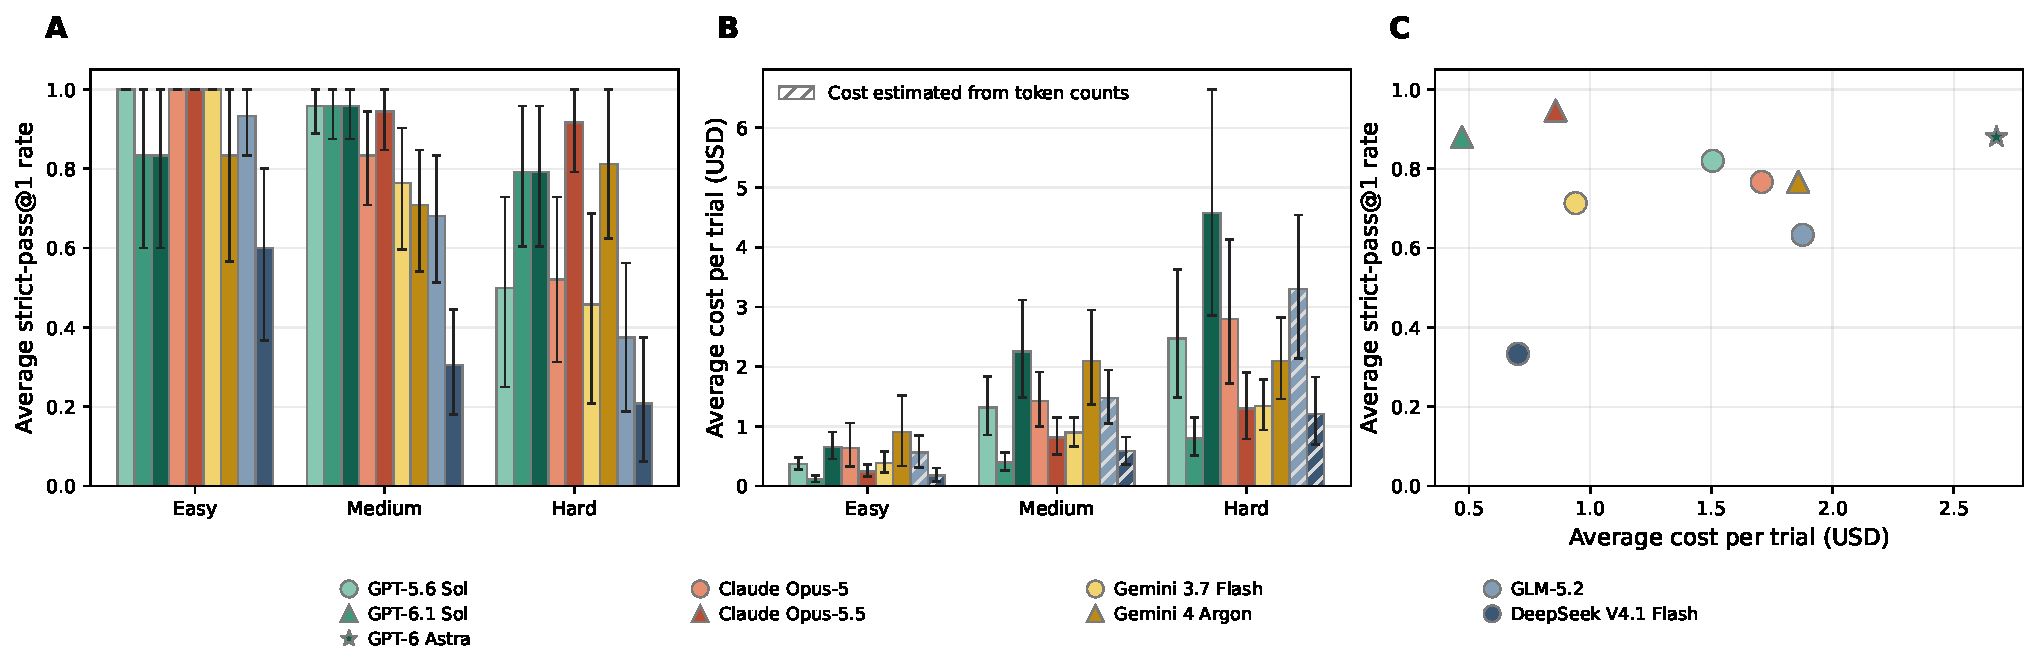
\includegraphics[width=\textwidth,trim=0bp 63bp 329bp 0bp,clip]{chapters/Ch7-Automating-ABFEP-calculations-with-AI-agents/figures/figure_3.pdf}\par
  \medskip
  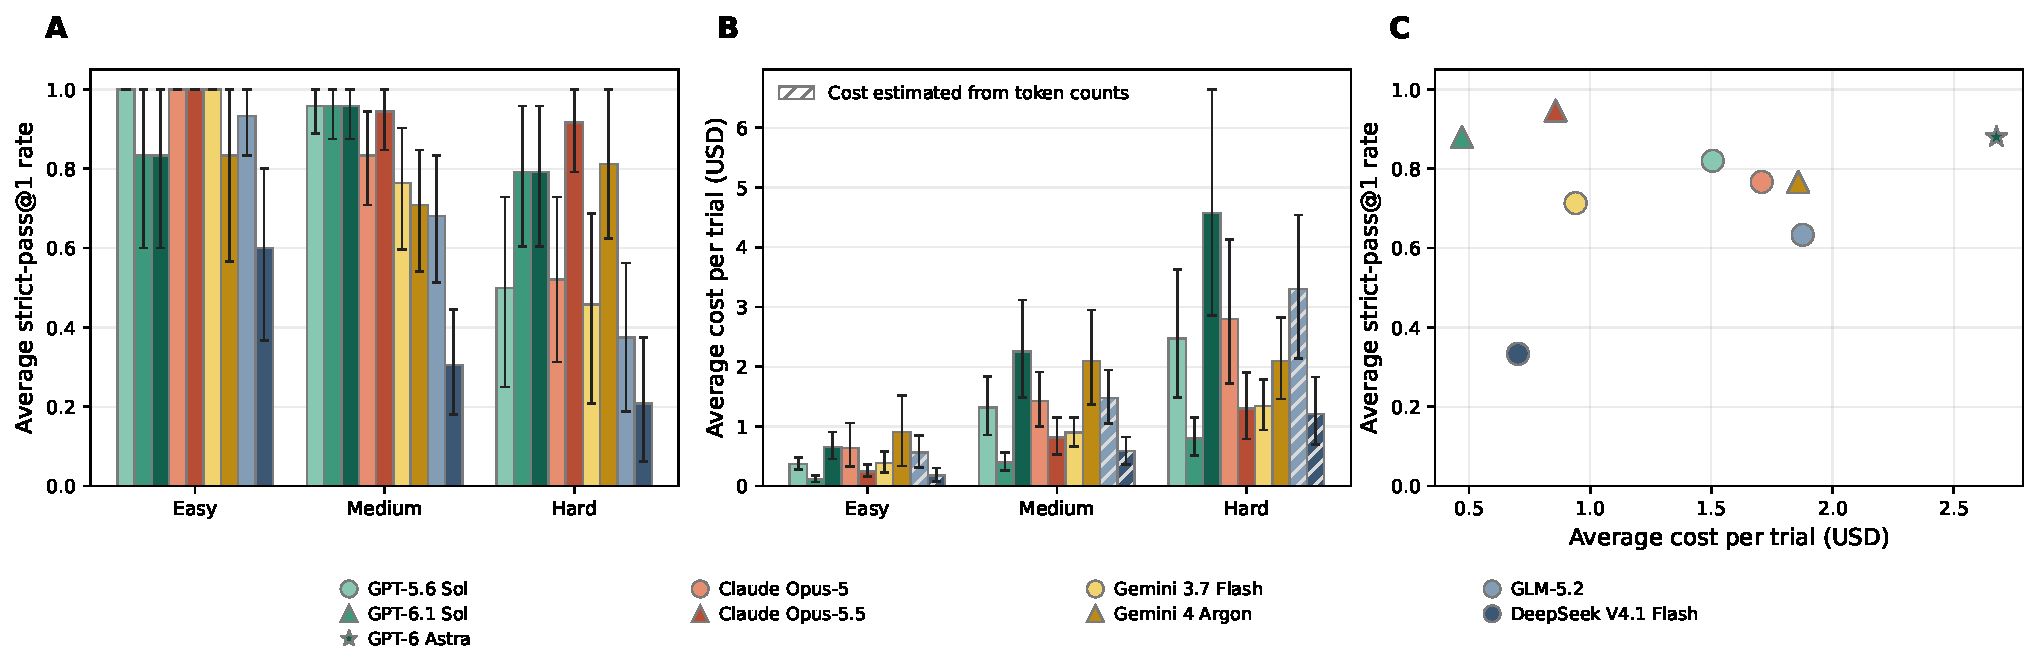
\includegraphics[width=\textwidth,trim=157bp 0bp 151bp 272bp,clip]{chapters/Ch7-Automating-ABFEP-calculations-with-AI-agents/figures/figure_3.pdf}
  \caption[Coding-agent performance and cost by task difficulty on MDArena.]{Performance and cost of nine coding-agent configurations on MDArena by task difficulty. (A) Mean Strict-Pass@1. (B) Mean cost per trial. A strict pass requires correctness and process scores of one. Error bars show 95\% task-bootstrap confidence intervals. Striped bars indicate costs estimated from exported token counts. GLM-5.2 estimates use its supplied mean cost at 1~GBP~=~1.36~USD. DeepSeek V4.1 Flash estimates use Vertex AI list prices.}
  \label{fig:difficulty_cost}
  \label{fig:cost-by-difficulty}
\end{figure}

\begin{figure}[htbp]
\centering
  % Isolate panel C without its panel label and repeat the model legend.
  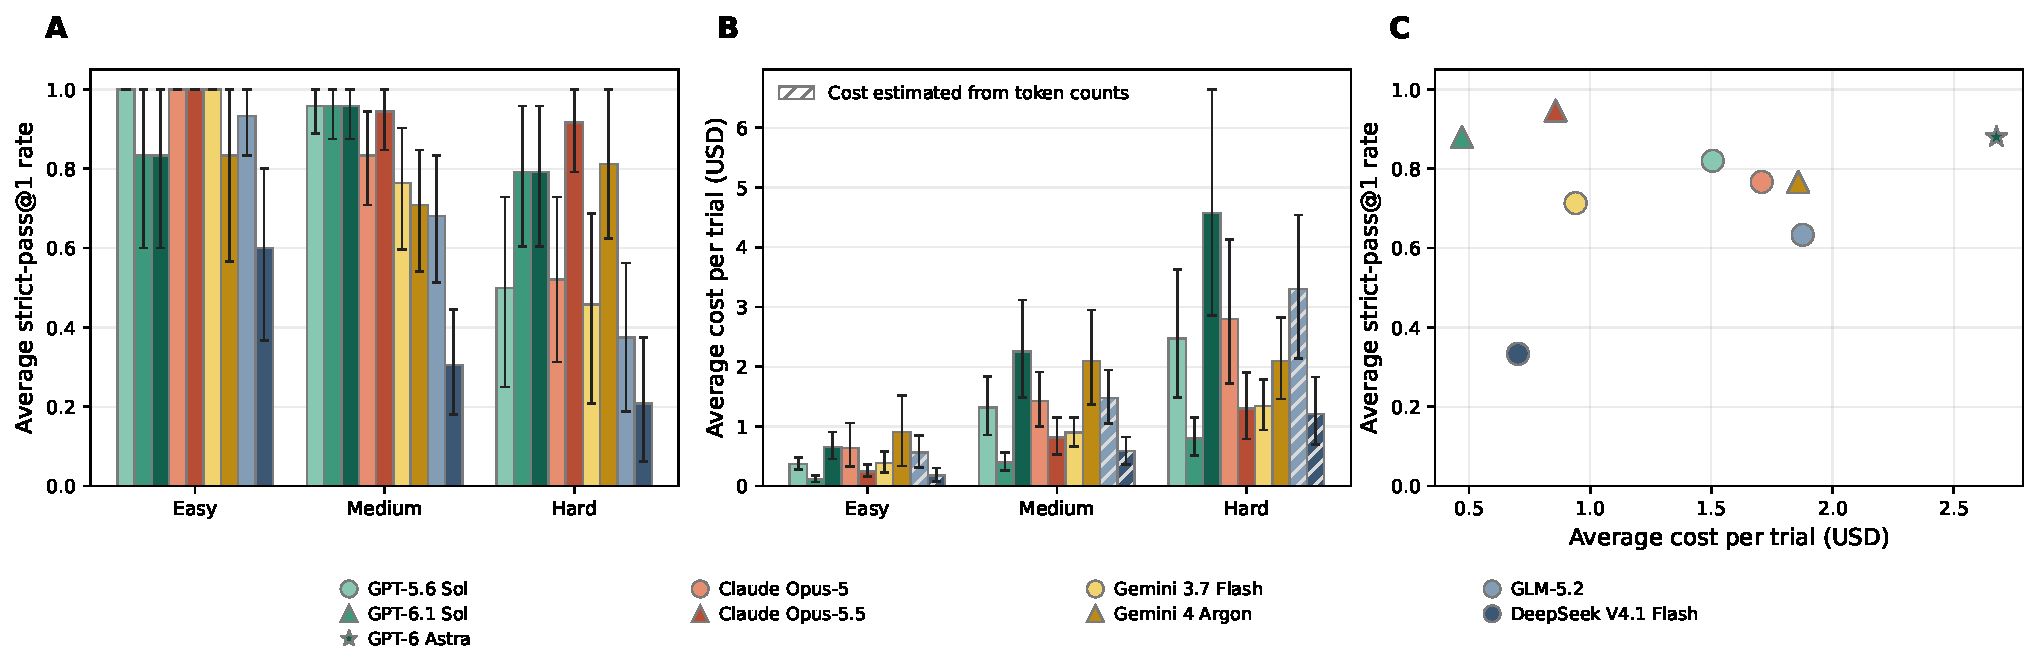
\includegraphics[width=0.8\textwidth,trim=650bp 50bp 0bp 26bp,clip]{chapters/Ch7-Automating-ABFEP-calculations-with-AI-agents/figures/figure_3.pdf}\par
  \medskip
  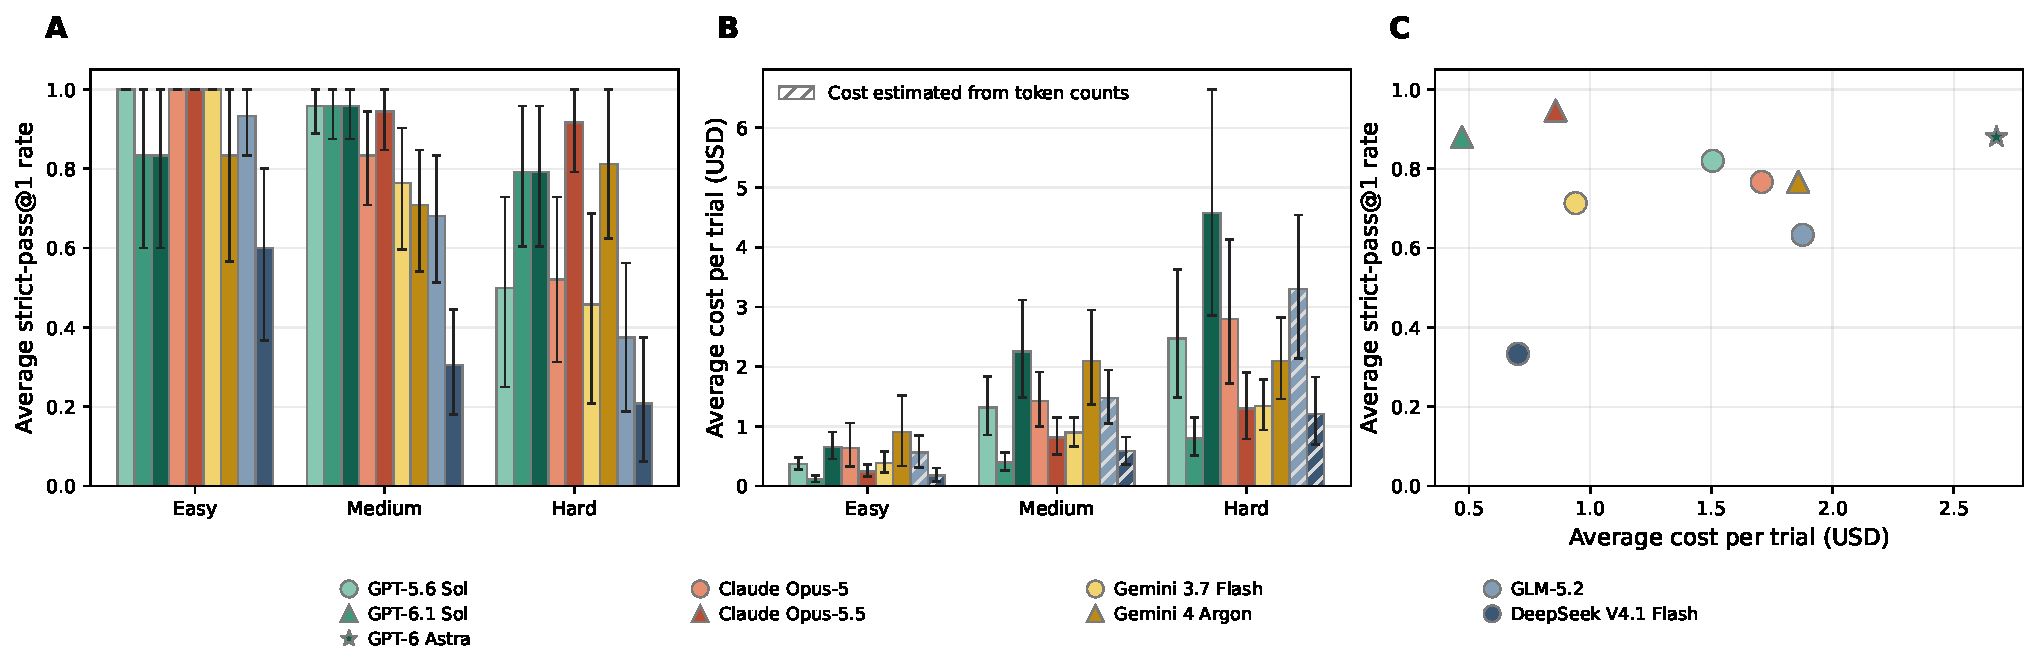
\includegraphics[width=\textwidth,trim=157bp 0bp 151bp 272bp,clip]{chapters/Ch7-Automating-ABFEP-calculations-with-AI-agents/figures/figure_3.pdf}
  \caption[Overall coding-agent performance against cost on MDArena.]{Overall mean Strict-Pass@1 against mean cost per trial for nine coding-agent configurations on MDArena. A strict pass requires correctness and process scores of one. GLM-5.2 costs are estimated using its supplied mean cost at 1~GBP~=~1.36~USD. DeepSeek V4.1 Flash costs are estimated from exported token counts using Vertex AI list prices.}
  \label{fig:overall_cost_performance}
\end{figure}

\subsection[Performance on hard tasks]{Frontier models tested solve previously intractable hard tasks}

The latest generation of frontier LLMs tested (Gemini 4 Argon, Opus-5.5, GPT-6.1 Sol and GPT-6 Astra) showed substantial gains over their predecessors, particularly on hard tasks. Strict-Pass@1 on hard tasks rose from 45.8\% for Gemini 3.7 Flash to 81.3\% for Gemini 4 Argon (22/48 to 39/48 attempts), from 50.0\% for GPT-5.6 Sol to 79.2\% for GPT-6.1 Sol (24/48 to 38/48), and from 52.1\% for Opus-5 to 91.7\% for Opus-5.5 (25/48 to 44/48). GPT-6 Astra likewise achieved 79.2\% (38/48). Opus-5.5, GPT-6.1 Sol and GPT-6 Astra passed a shared set of 12 hard tasks in all three attempts. Opus-5.5 passed 14 hard tasks consistently and all 16 at least once, while Sol and Astra each passed 14/16 at least once. Shared successes go beyond typical analysis tasks and included enhanced-sampling preparation (Tasks 28 and 30), ligand and residue parameterization (Tasks 24 and 47), and force-field repair (Task 46). They also included scientific assessment: evaluating the suitability of a PCA-derived collective variable (Task 22) and assessing protein placement relative to the lipid bilayer (Task 45).


\subsection{Failures persist despite improved hard-task performance}

Despite improvements on hard tasks, failures persisted even on simpler tasks. Gemini 4, GPT-6.1 Sol and GPT-6 Astra each passed only 25 of 30 easy trials, while most other frontier models passed all 30. All three models failed every attempt at converting a glycosylated insulin system from AMBER to GROMACS (Task 11): the delivered files lacked the periodic box vectors GROMACS needs to process the system for energy minimization. Each also failed two of three attempts to scale ion charges in a water-decane system (Task 18). Although they correctly scaled the ions used by the system, they also modified unused parameters. Astra and Gemini 4 Argon changed an unused alternative sodium type, \texttt{opls\_405}; Sol additionally changed \texttt{opls\_709}, a chloride site belonging to a reaction transition-state model. These changes violated a correctness check requiring the parameters of all other non-target moieties to remain unchanged. In addition, Gemini 4 Argon timed out in the Harbor environment more often than any other model (24 of 150 trials, compared with 6 of 150 for the next highest, GLM), as it spent extended periods troubleshooting and investigating errors.

Failures in medium and hard tasks mostly belonged to membrane protein setup or free energy perturbation. The failures came from Tasks~39 and~32. In Task~39, the agent was tasked with setting up GROMACS ABFE calculations for a set of charged ligands binding to the dopamine D3 receptor. All three attempts by every frontier model lacked a completed charge-treatment strategy. As the ligand's charge changed from $+1$ to $0$, the system's total charge changed by $-1e$. The agents acknowledged the resulting electrostatic concern but deferred its treatment, so they were penalized for leaving a charged system that might introduce artifacts. This case therefore highlights the importance of specifying scientific edge cases in complex workflows. The second was the DHODH OpenFE network, where Opus-5.5 failed one of three attempts: it took longer than expected to align the 15 ligands, leading to a timeout that left the final network and transformation files undelivered.

Membrane-protein preparation remained particularly challenging. Across five hard membrane-preparation tasks, GPT-6.1 Sol and Astra each passed 33.3\% of attempts (5/15), compared with 73.3\% (11/15) for Opus-5.5 and 80\% (12/15) for Gemini 4 Argon. Insufficient lipid packing dominated the failures in membrane protein preparation tasks: most agents removed whole overlapping lipids, which often left underfilled exterior regions without subsequent repacking. However, although Opus-5.5 passed the lipid-packing checks in 14/15 trials for membrane tasks, it exhibited other failures resulting from incorrect final assembly despite valid intermediate work. In two of three mGlu5R system setup (task 25) trials, Opus-5.5 preserved the ligand’s binding pose in an intermediate structure, then shifted the receptor and ligand by different amounts during final assembly. The ligand ended up 30.2 and 37.8 Å from the nearest protein atom, failing the correctness checks for binding pocket geometry. Another assembly failure occurred in PepT2 system preparation (task 29), where the final structure still contained severe clashes. One ligand carbon and one lipid carbon were only 1.37 Å apart, far too close for two nonbonded carbon atoms, causing an infinite force during minimization and therefore failing the checks.

\begin{figure}[htbp]
\centering
  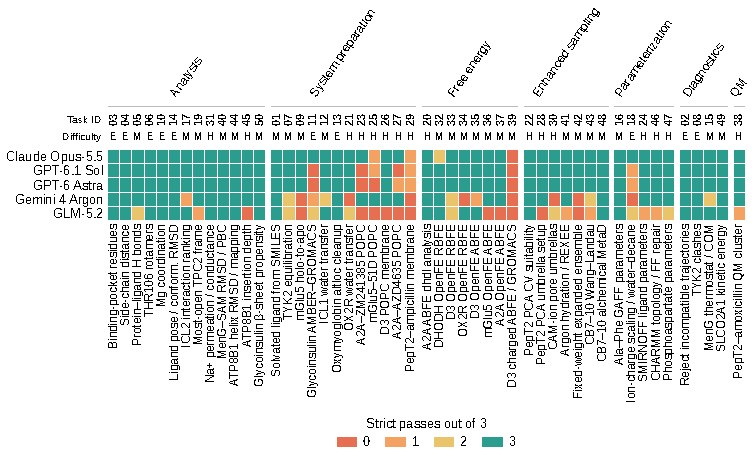
\includegraphics[width=\textwidth]{chapters/Ch7-Automating-ABFEP-calculations-with-AI-agents/figures/figure_5/variants/task_success_angled.pdf}
  \caption[Task-level strict-pass counts on MDArena.]{Strict passes across three attempts per task for five coding-agent configurations on all 50 MDArena tasks, grouped by task type. Colours indicate zero to three strict passes. A strict pass requires completion and full correctness and process scores. E/M/H indicate easy, medium, and hard tasks; QM denotes quantum chemistry.}
\end{figure}

\begin{figure}[htbp]
\centering
  % Place the two assembly examples side by side, relabelling original B/C as A/B.
  \begin{minipage}[t]{0.48\textwidth}
    \raggedright
    \textsf{\textbf{A}}\par
    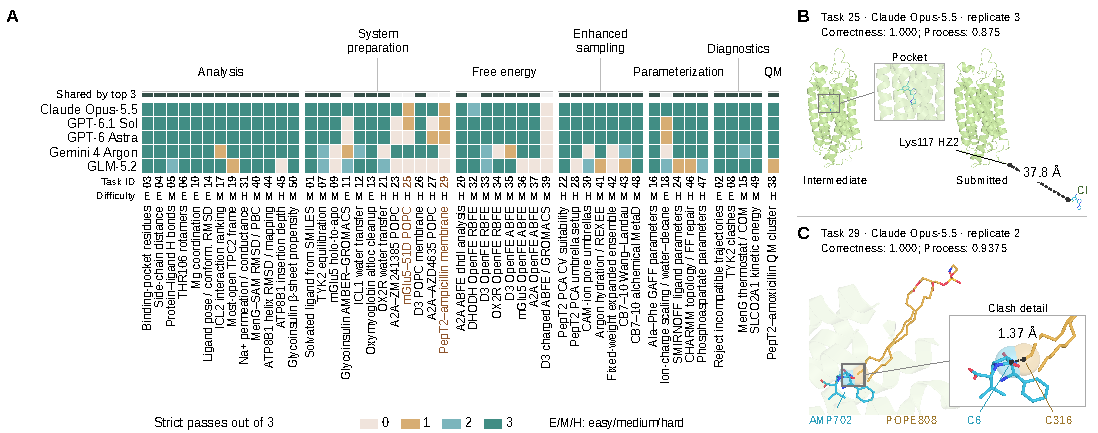
\includegraphics[width=\linewidth,trim=381bp 105bp 0bp 20bp,clip]{chapters/Ch7-Automating-ABFEP-calculations-with-AI-agents/figures/task_success_examples_source.pdf}
  \end{minipage}\hfill
  \begin{minipage}[t]{0.48\textwidth}
    \raggedright
    \textsf{\textbf{B}}\par
    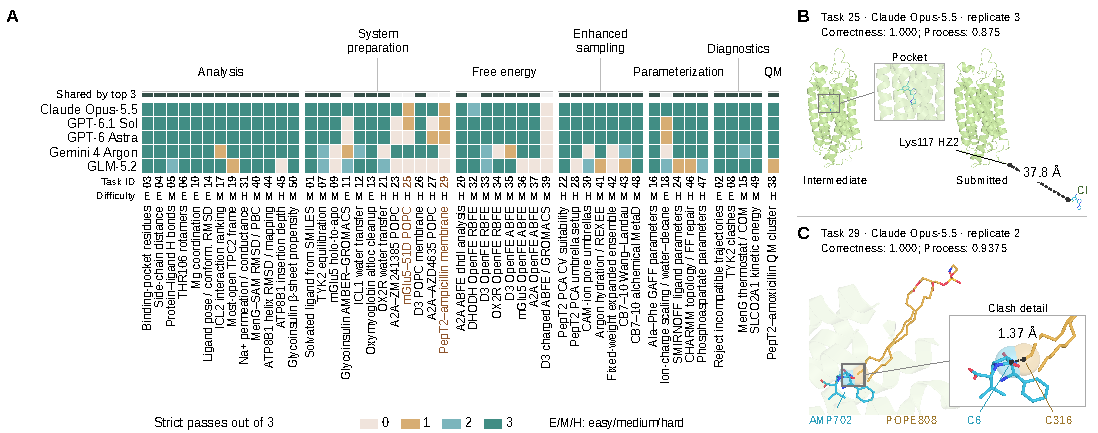
\includegraphics[width=\linewidth,trim=381bp 0bp 0bp 124bp,clip]{chapters/Ch7-Automating-ABFEP-calculations-with-AI-agents/figures/task_success_examples_source.pdf}
  \end{minipage}
  \caption[Examples of molecular-system assembly failures.]{Two assembly failures from Claude Opus-5.5. (A) Task~25, replicate~3: the intermediate mGlu5--51D structure retains the binding pose, whereas the submitted assembly has a nearest ligand--protein atom separation of 37.8~\AA{}, accounting for periodic boundaries. The receptor views have matched orientation and scale; the inset enlarges the intermediate pocket. Correctness and process scores were 1.000 and 0.875, respectively. (B) Task~29, replicate~2: ligand AMP702 C6 and lipid POPE808 C316 are separated by a 1.37~\AA{} nonbonded contact. The inset enlarges the contact with transparent carbon van der Waals spheres. Correctness and process scores were 1.000 and 0.9375, respectively. This contact is not established as the unique cause of the non-finite force reported during minimization.}
\end{figure}

\subsection{Cost effectiveness of different models}

Cost per successful trial is a key consideration for industrial adoption. Mean cost rose with task difficulty (Fig.~\ref{fig:difficulty_cost}B), reflecting longer agent runtimes and greater token usage. The latest generation of models substantially reduced cost while improving success (Fig.~\ref{fig:difficulty_cost}B). Mean cost per trial fell by 49.8\% for Claude Opus-5.5 relative to Opus-5 (\$1.71 to \$0.86) and by 68.8\% for GPT-6.1 Sol relative to GPT-5.6 Sol (\$1.51 to \$0.47). Gemini 4 Argon was an exception, nearly doubling the cost of Gemini 3.7 Flash (\$1.86 versus \$0.94) by processing 31\% more input tokens despite fewer tool calls (59 versus 65), though its strict pass rate also rose (71.3\% to 76.7\%), with an exceptional improvement on hard tasks (45.8\% to 81.3\%). We also see that higher cost did not guarantee better performance (Fig.~\ref{fig:overall_cost_performance}): the flagship GPT-6 Astra cost \$2.68 per trial, 5.7 times that of GPT-6.1 Sol, yet only matched its 88.0\% strict pass rate. Overall, GPT-6.1 Sol had the lowest cost per strict pass (\$0.53), while Claude Opus-5.5 achieved the highest strict pass rate for an additional \$0.39 per trial.



\subsection{Behavioural differences between model families}

Manual inspection of the MDArena trajectories showed clear differences in how agents planned, executed, and validated their work. Models from the same lab behaved alike. 

GPT-6 Astra and GPT-6.1 Sol, run in the shared Codex harness, grouped related operations into batches and validated intermediate results before proceeding. Across full cohorts, Astra used a median of 12.5 calls and 4.1 minutes per trial, and Sol 14 calls and 3.9 minutes. This differed from the behaviour of Claude Opus 5.5, which typically moved from a short inspection to a script that produced the requested files, followed by an end-to-end check. It was quick to make and document reasonable assumptions, and had the lowest median tool count and execution time (11 calls, 2.0 minutes). For example, when converting an AMBER system with no periodic box to GROMACS (Task 11), it added a box to the delivered structure and disclosed the choice, passing all three repeats. Astra and Sol used temporary boxes only for validation and delivered structures with zero box vectors, which failed the verifier’s periodic preprocessing check. 

Gemini 4 Argon, by contrast, prioritised exploration over delivery, spending more of its workflow inspecting files, probing library behaviour, and updating plans. It used the to-do tool in 123 of 150 trials, with a median of 53 calls and 18.5 minutes. On the ProLIF interaction analysis (Task 17), two repeats had already printed the correct top-ten interactions when the agent kept investigating residue numbering and export details; both hit the 15-minute limit without saving the requested CSV or summary. GLM-5.2 also explored extensively, mainly through small shell and Python experiments (to-do tool in 62 of 150 trials; median 35 calls and 17.5 minutes). This paid off on some tasks, such as Task 34, where GLM resolved failed imports and topology-loading problems, built the OpenFE network, and confirmed the saved transformations could be reloaded, passing all three repeats with 106–140 calls each. Gemini timed out on all three without delivering the network.

\section{Conclusion}

Performance on MDArena demonstrates substantial progress towards reliable automation of molecular dynamics workflows. Claude Code–Opus-5.5 achieved the highest Strict-Pass@1 rate at 94.7\% (142/150 trials), followed by GPT-6.1 Sol and GPT-6 Astra at 88.0\% each (132/150). Improvements extended to demanding workflows: Opus-5.5 passed 91.7\% of hard-task attempts (44/48), compared with 52.1\% (25/48) for Opus-5. Nevertheless, even Opus-5.5 failed at least one of three attempts on 8.0\% of tasks (4/50), with all three attempts failing on 2.0\% (1/50). These results support integrating coding agents into clearly specified, bounded research workflows with independent validation. They do not yet establish dependable execution of entire computational research projects. Closing the remaining gap between high aggregate performance and consistent scientific correctness remains a priority for the next generation of agents.

MDArena has several limitations. The process verifier relies on an LLM judge, introducing model dependence despite task-specific, criterion-anchored rubrics. The tasks originate from a single research group and may reflect its expertise and conventions rather than the full diversity of MD practice. Task selection also deliberately emphasized workflows expected to expose agent failure modes; the reported success rates therefore should not be interpreted as estimates across all routine MD tasks. Furthermore, results characterize model–harness configurations under specified computational resources and time limits, so differences cannot be attributed solely to the underlying models.

The benchmark primarily evaluates system preparation and analysis rather than long-running, stochastic production simulations. Extending evaluation to end-to-end simulation workflows is an important direction, but will require assessing protocol validity and statistical adequacy without treating agreement with a particular stochastic trajectory as the criterion for success. MDArena is intended as an extensible, longitudinal evaluation framework: the current task suite provides a versioned reference point, while future releases can incorporate additional systems, methods, and community-contributed workflows as agent capabilities advance.


\section*{Data availability}


The MDArena benchmark, including task definitions and inputs, Docker specifications, verifier implementations, reference solutions, and evaluation configurations, is publicly available at
\url{https://github.com/weitse-hsu/MDArena}. The repository also provides instructions for reproducing
the reported results. The version corresponding to this manuscript is archived as v1.
